\documentclass[a4paper,12pt]{article}



\usepackage{graphicx}

\title{How to build a geodesic dome}
\author{Andr\'{e} Franz}
\date{}


\begin{document}
\maketitle

\section{The basics}
From Wikipedia:
\begin{quote}
A geodesic dome is a spherical or partial-spherical shell structure or lattice shell based on a network of great circles (geodesics) on the surface of a sphere. The geodesics intersect to form triangular elements that have local triangular rigidity and also distribute the stress across the structure. When completed to form a complete sphere, it is a geodesic sphere. [...]

Typically a geodesic dome design begins with icosahedron inscribed in a hypothetical sphere, tiling each triangular face with smaller triangles, then projecting the vertices of each tile to the sphere. The endpoints of the links of the completed sphere are the projected endpoints on the sphere's surface. If this is done exactly, sub-triangle edge lengths take on many different values, requiring links of many sizes. [...]
\end{quote}

As mentioned above, a geodesic dome design is usually based on a regular icosahedron (see Figure \ref{fig:icosahedron}), which is a convex polyhedron with 20 faces, 30 edges and 12 vertices. The 20 faces are \textbf{equilateral} triangles.

\begin{figure}
	\centering
	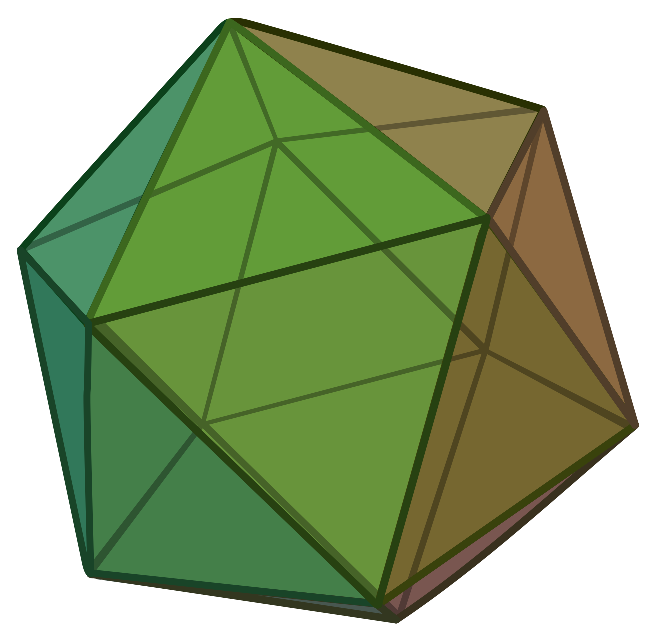
\includegraphics[width=0.5\linewidth]{../images/icosahedron.eps}
	\caption{Regular icosahedron.\newline(Source: https://commons.wikimedia.org/wiki/File:Icosahedron.svg)}
	\label{fig:icosahedron}
\end{figure}

To get a more \emph{sperical} look, the triangles of the icosahedron are tiled with smaller triangles (see Figure \ref{fig:tiling}). This is done by deviding the egdes of the triangle into smaller edges with equal length. The number of these \emph{edges} per original edge of the icosahedron is called \emph{frequency} of the dome. The original triangle of the icosahedron has of course only 1 edge, the frequency is therefore \textbf{1V} (see Figure \ref{fig:tiling} a)). If the original edge is devided into \textbf{two} smaller equal edges it is called frequency \textbf{2V} (see Figure \ref{fig:tiling} b)); if the original edge is devided into \textbf{three} smaller equal edges it is called frequency \textbf{3V} (see Figure \ref{fig:tiling} c)), and so on.

\begin{figure}
	\centering
	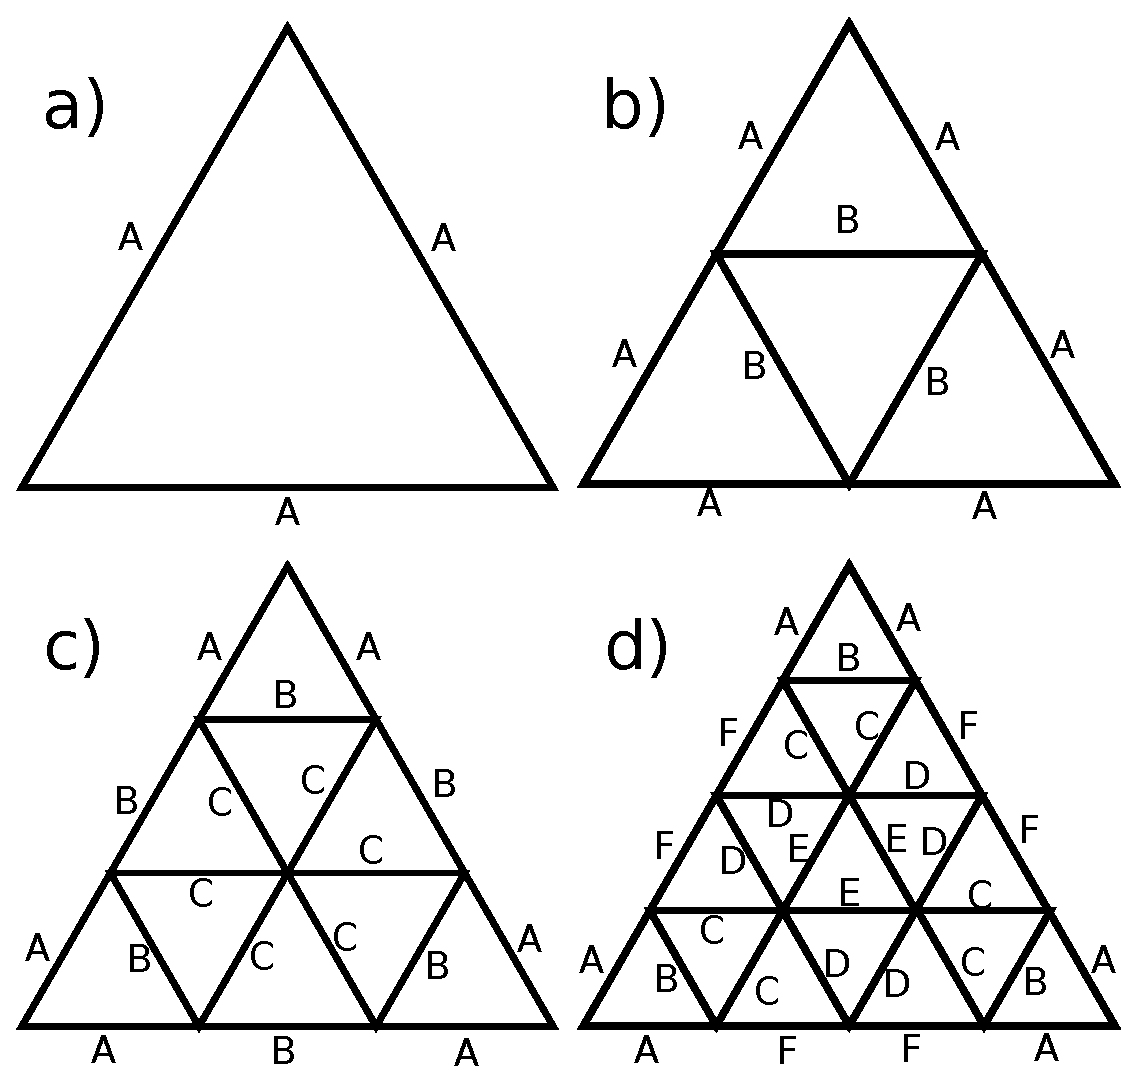
\includegraphics[width=0.7\linewidth]{../images/triangle_tiling.eps}
	\caption{Tiling of the triangle of the icosahedron. Subfigure a) shows the original triangle of the icosahedron (1V). In subfigure b) the triangle is tiled into four smaller triangles (2V). In subfigure c) the triangle is tiled into nine smaller triangles (3V) and in subfigure d) the triangle is tiled into 16 smaller triangles (4V).}
	\label{fig:tiling}
\end{figure}

These smaller tiles are still equilateral triangles, but also still located in the flat area of the original triangle of the icosahedron. Only the vertices of the original triangle of the icosahedron are located on circumscribed sphere, but not the vertices of the smaller tiles. To achive a more \emph{sperical} look it is of course necessary to project also the vertices of the smaller tiles on to the circumscribed sphere. Due to this projection the lengths of the edges of the smaller tiles will change. The projected tiles are no longer equilateral anymore. This is shown in Figure \ref{fig:projection}. 

\begin{figure}
	\centering
	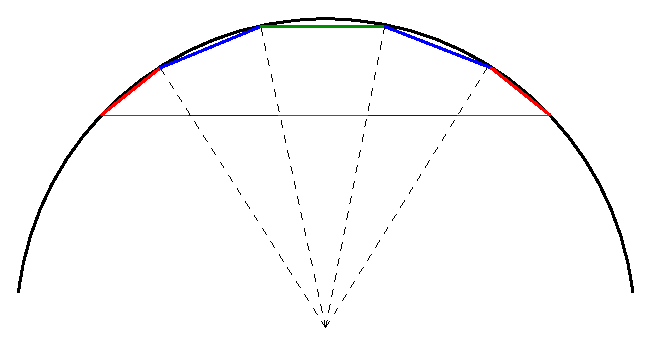
\includegraphics[width=0.7\linewidth]{../images/projection.eps}
	\caption{Five equilateral edges are projected to the circumscribed circle. After projection the edges will have different lengths.}
	\label{fig:projection}
\end{figure}

To calculate the new lengths of the edges of the smaller tiles some trigonometric magic is needed. However, there are a lot of websites, where people have already done this work and which provide so called \emph{strut factors}. The only thing one has to do, is to chose a frequency and the desired radius of the dome. The radius is than multiplied with the strut factors to get the different lengths of the edges of the tiles. Table \ref{tab:strut_factors} give the strut factors for geodesic domes with the frequencies 1V, 2V, 3V and 4V.


\begin{table}
	\centering
	\caption{Strut factors.}
	\begin{tabular}{l|cccccc}
strut	&	1V		& 2V		& 3V		& 4V				\\	\hline
	A	& 1.05146	& 0.54653	& 0.34862	& 0.25318		\\
	B	&			& 0.61803	& 0.40355	& 0.29524		\\
	C	&			&			& 0.41241	& 0.29453		\\
	D	&			&			&			& 0.31287		\\
	E	&			&			&			& 0.32492		\\
	F	&			&			&			& 0.29859		
	\end{tabular}
	\label{tab:strut_factors}
\end{table}

\section{Building a 4V geodesic dome}
To get a dome which is exact one half of a sphere, we need to extend the triangle in Figure \ref{fig:tiling} d) to the one seen in Figure \ref{fig:tiling_4v}.

\begin{figure}
	\centering
	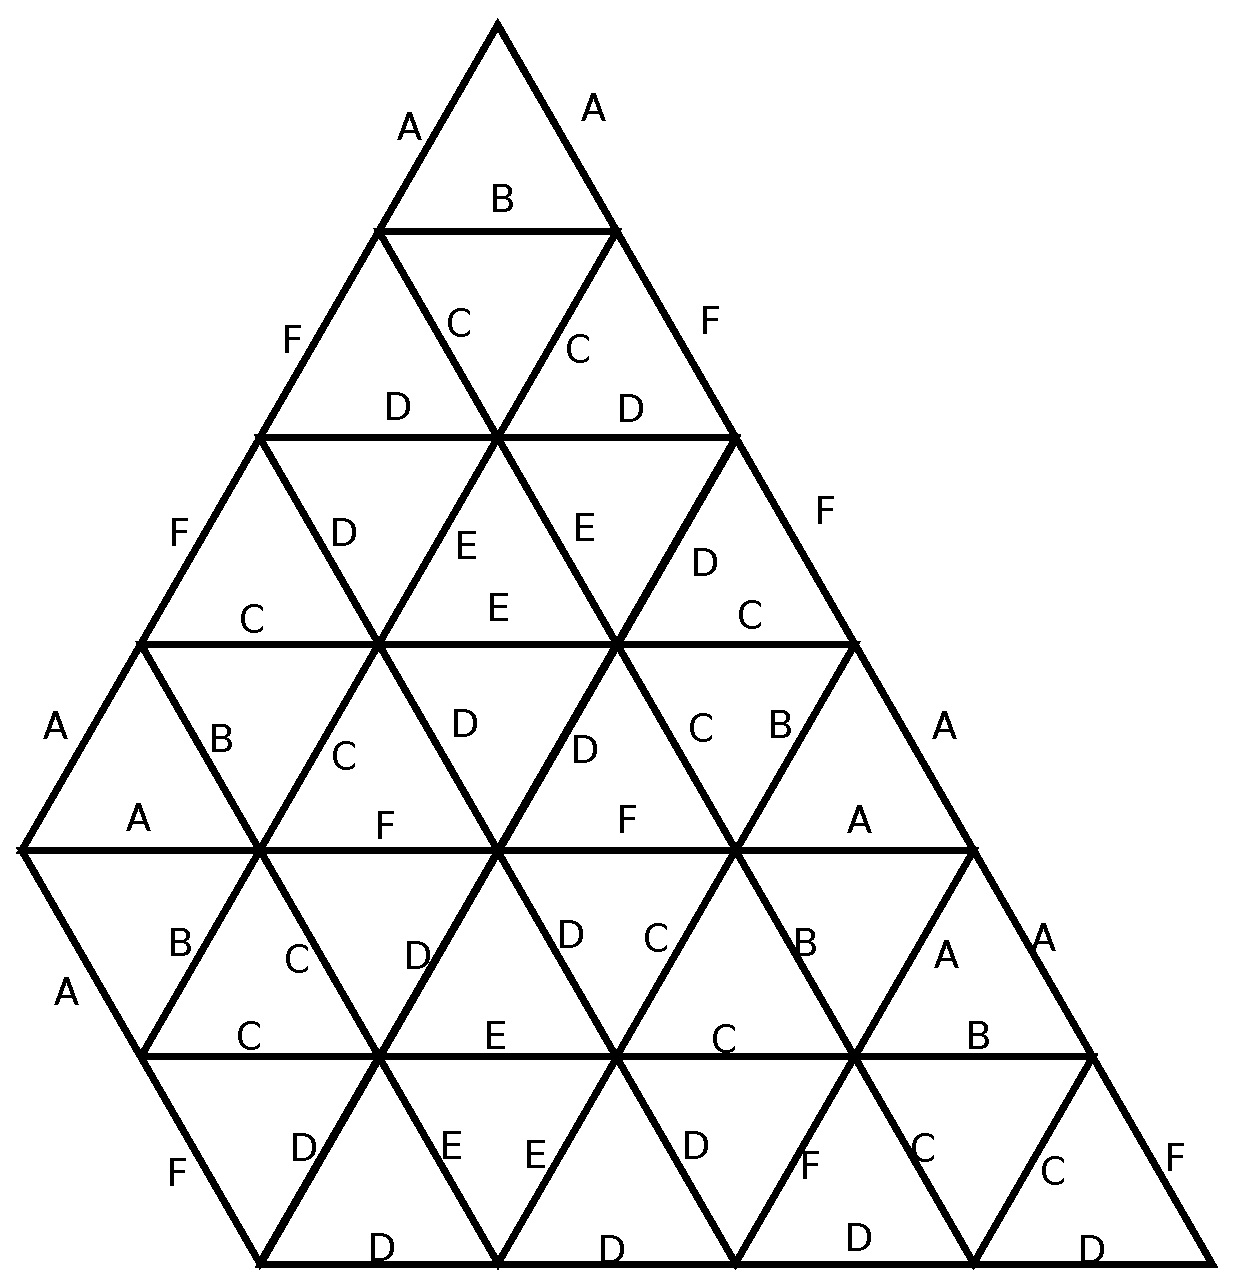
\includegraphics[width=0.7\linewidth]{../images/tiling_4v.eps}
	\caption{1/5 of a 4V geodesic dome.}
	\label{fig:tiling_4v}
\end{figure}

For a radius of 10 meters we can just calculate all the length with the given factors in Table \ref{tab:strut_factors}. The resulting lengths are given in Table \ref{tab:length4v}.

\begin{table}
	\centering
	\caption{Strut lengths of a 4V dome with a radius of 10 meters.}
	\begin{tabular}{l|ll}
strut	& factor	& length				\\	\hline
	A	& 0.25318	& 253.18 cm		\\
	B	& 0.29524	& 295.24 cm	\\
	C	& 0.29453	& 294.53 cm	\\
	D	& 0.31287	& 312.87 cm		\\
	E	& 0.32492 	& 324.92 cm		\\
	F	& 0.29859	& 298.59 cm	
	\end{tabular}
	\label{tab:length4v}
\end{table}

\end{document}
